\documentclass{standalone}
\usepackage{tikz}
\begin{document}
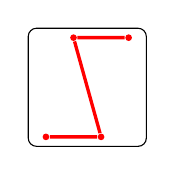
\begin{tikzpicture}[scale=1.5]
  % draw rounded cell boxes
  \draw[rounded corners=3pt] (0,0) rectangle (1,1);
  % draw black chords for chord_row_cells
  \node[circle, fill=red, inner sep=0.03cm] (obs4430386608_pt0) at (0.15,0.08) {};
  \node[circle, fill=red, inner sep=0.03cm] (obs4430386608_pt1) at (0.3833333333333333,0.9200000000000002) {};
  \node[circle, fill=red, inner sep=0.03cm] (obs4430386608_pt2) at (0.6166666666666666,0.08) {};
  \node[circle, fill=red, inner sep=0.03cm] (obs4430386608_pt3) at (0.85,0.9200000000000002) {};
  \draw[red, line width=1.2pt] (obs4430386608_pt0) -- (obs4430386608_pt2) -- (obs4430386608_pt1) -- (obs4430386608_pt3);
\end{tikzpicture}
\end{document}